% answers.tex —— 2005 年·春季北京卷·文科 · 参考答案与详细解析片段
% 由 tools/generate_projects.py 依来源总账自 2005/2005_数学真题_春季北京文_试题.md + 2005/2005_数学真题_春季北京文_解析正文.md + 2005/2005_数学真题_春季北京文_答案要点.md 生成，勿手改（改源 MD 后重跑）


本解析依据固定题面上的题干、选项和图示逐题独立推导，证据等级 D；不代表官方答案或官方解析。

\gkpart{一、选择题}

\begin{answer}
\gksolhead{1}{}

\textbf{题目}：

$i-2$ 的共轭复数是\mbox{（　　）}。

（A）$2+i$　　（B）$2-i$　　（C）$-2+i$　　（D）$-2-i$

\Needspace{4\baselineskip}
\textbf{解析}

先化简 $i-2=-2+i$，其共轭复数为 $-2-i$，对应 D。

\gkanswer{答案：D，$-2-i$}

\end{answer}
\begin{answer}
\gksolhead{2}{}

\textbf{题目}：

函数 $y=|\log_2 x|$ 的图象是\mbox{（　　）}。
\nopagebreak[4]
\begin{center}% Source-page vector redraw of the four function-graph options.
% Curves preserve visible topology only; coordinates are schematic.
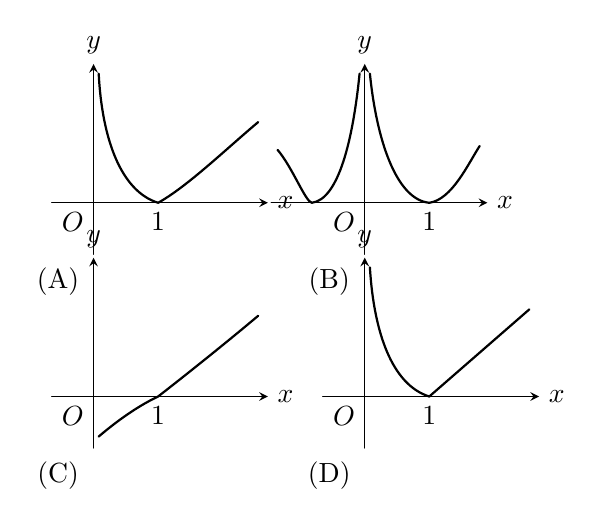
\begin{tikzpicture}[>=stealth, line cap=round, line join=round, scale=.82]
% Option A
\begin{scope}[shift={(0,0)}]
  \draw[->] (-.65,0)--(2.7,0) node[right] {$x$}; \draw[->] (0,-.8)--(0,2.15) node[above] {$y$};
  \node[below left] at (0,0) {$O$}; \node[below] at (1,0) {$1$}; \node at (-.55,-1.22) {(A)};
  \draw[thick] (.08,2.0) .. controls (.13,1.0) and (.42,.18) .. (1,0) .. controls (1.45,.25) and (2.05,.83) .. (2.55,1.25);
\end{scope}
% Option B
\begin{scope}[shift={(4.2,0)}]
  \draw[->] (-1.45,0)--(1.9,0) node[right] {$x$}; \draw[->] (0,-.8)--(0,2.15) node[above] {$y$};
  \node[below left] at (0,0) {$O$}; \node[below] at (1,0) {$1$}; \node at (-.55,-1.22) {(B)};
  \draw[thick] (-1.35,.82) .. controls (-1.12,.55) and (-.92,.02) .. (-.82,0) .. controls (-.4,.05) and (-.18,1.0) .. (-.08,2.0);
  \draw[thick] (.08,2.0) .. controls (.18,1.0) and (.48,.05) .. (1,0) .. controls (1.35,.05) and (1.6,.6) .. (1.78,.88);
\end{scope}
% Option C
\begin{scope}[shift={(0,-3.0)}]
  \draw[->] (-.65,0)--(2.7,0) node[right] {$x$}; \draw[->] (0,-.8)--(0,2.15) node[above] {$y$};
  \node[below left] at (0,0) {$O$}; \node[below] at (1,0) {$1$}; \node at (-.55,-1.22) {(C)};
  \draw[thick] (.08,-.62) .. controls (.28,-.45) and (.62,-.18) .. (1,0) .. controls (1.45,.35) and (2.05,.83) .. (2.55,1.25);
\end{scope}
% Option D
\begin{scope}[shift={(4.2,-3.0)}]
  \draw[->] (-.65,0)--(2.7,0) node[right] {$x$}; \draw[->] (0,-.8)--(0,2.15) node[above] {$y$};
  \node[below left] at (0,0) {$O$}; \node[below] at (1,0) {$1$}; \node at (-.55,-1.22) {(D)};
  \draw[thick] (.08,2.0) .. controls (.14,1.0) and (.42,.18) .. (1,0);
  \draw[thick] (1,0)--(2.55,1.35);
\end{scope}
\end{tikzpicture}
\end{center}
\nopagebreak[4]
\Needspace{4\baselineskip}
\textbf{解析}

函数 $y=|\log_2x|$ 的定义域为 $x>0$。当 $0<x<1$ 时 $y=-\log_2x$，随 $x$ 增大而下降；在 $x=1$ 取最小值 $0$；当 $x>1$ 时 $y=\log_2x$，递增。因此图像只在 $x>0$ 有定义，在 $(1,0)$ 处触及 $x$ 轴，左支趋于正无穷，与 A 相符。

\gkanswer{答案：A}

\end{answer}
\begin{answer}
\gksolhead{3}{}

\textbf{题目}：

下列命题中，正确的是\mbox{（　　）}。

（A）经过不同的三点有且只有一个平面

（B）分别在两个平面内的两条直线一定是异面直线

（C）垂直于同一个平面的两条直线是平行直线

（D）垂直于同一个平面的两个平面平行

\Needspace{4\baselineskip}
\textbf{解析}

两条直线若都垂直于同一平面，其方向都平行于该平面的法向量，因而两直线平行。A 未排除三点共线；B 中分别位于两平面内的直线可以相交或平行；D 中两个平面可相交且都垂直于第三个平面，故只有 C 必然成立。

\gkanswer{答案：C}

\end{answer}
\begin{answer}
\gksolhead{4}{}

\textbf{题目}：

如果函数 $f(x)=\sin(\pi x+\theta)$（$0<\theta<2\pi$）的最小正周期是 $T$，且当 $x=2$ 时取得最大值，那么\mbox{（　　）}。

（A）$T=2,\ \theta=\dfrac{\pi}{2}$　　（B）$T=1,\ \theta=\pi$

（C）$T=2,\ \theta=\pi$　　（D）$T=1,\ \theta=\dfrac{\pi}{2}$

\Needspace{4\baselineskip}
\textbf{解析}

函数 $f(x)=\sin(\pi x+\theta)$ 的最小正周期满足 $\pi T=2\pi$，故 $T=2$。$x=2$ 取最大值时 $\sin(2\pi+\theta)=1$，结合 $0<\theta<2\pi$ 得 $\theta=\pi/2$，对应 A。

\gkanswer{答案：A}

\end{answer}
\begin{answer}
\gksolhead{5}{}

\textbf{题目}：

设 $abc\ne0$，“$ac>0$”是“曲线 $ax^2+by^2=c$ 为椭圆”的\mbox{（　　）}。

（A）充分非必要条件　　（B）必要非充分条件

（C）充分必要条件　　（D）既非充分又非必要条件

\Needspace{4\baselineskip}
\textbf{解析}

若 $ax^2+by^2=c$ 表示椭圆，且 $abc\ne0$，除以 $c$ 后两个平方项的系数 $a/c,b/c$ 均为正。特别地，$ac>0$，所以它是必要条件。反过来，$ac>0$ 并不限制 $b/c$ 的符号；若 $b/c<0$，方程不能表示椭圆。因此它不充分。

\gkanswer{答案：B，必要非充分条件}

\end{answer}
\begin{answer}
\gksolhead{6}{}

\textbf{题目}：

直线 $x+\sqrt{3}\,y-2=0$ 被圆 $(x-1)^2+y^2=1$ 所截得的线段的长为\mbox{（　　）}。

（A）$1$　　（B）$\sqrt{2}$　　（C）$\sqrt{3}$　　（D）$2$

\Needspace{4\baselineskip}
\textbf{解析}

\Needspace{5\baselineskip}
圆 $(x-1)^2+y^2=1$ 的圆心为 $(1,0)$，半径为 $1$。圆心到直线 $x+\sqrt3y-2=0$ 的距离是
\nopagebreak[4]
\[
d=\frac{|1-2|}{\sqrt{1+3}}=\frac12.
\]
\Needspace{5\baselineskip}
弦长为
\nopagebreak[4]
\[
2\sqrt{1-d^2}=2\sqrt{1-\frac14}=\sqrt3.
\]

\gkanswer{答案：C，$\sqrt3$}

\end{answer}
\begin{answer}
\gksolhead{7}{}

\textbf{题目}：

在 $\triangle ABC$ 中，已知 $2\sin A\cos B=\sin C$，那么 $\triangle ABC$ 一定是\mbox{（　　）}。

（A）直角三角形　　（B）等腰三角形　　（C）等腰直角三角形　　（D）正三角形

\Needspace{4\baselineskip}
\textbf{解析}

\Needspace{5\baselineskip}
三角形内角满足 $C=\pi-(A+B)$，所以 $\sin C=\sin(A+B)$。题设
\nopagebreak[4]
\[
2\sin A\cos B=\sin C
\]
\Needspace{5\baselineskip}
化为
\nopagebreak[4]
\[
\sin A\cos B=\cos A\sin B,
\]
即 $\sin(A-B)=0$。因 $A,B\in(0,\pi)$，故 $A-B=0$，即 $A=B$，三角形为等腰三角形。

\gkanswer{答案：B，等腰三角形}

\end{answer}
\begin{answer}
\gksolhead{8}{}

\textbf{题目}：

\Needspace{5\baselineskip}
若不等式

\nopagebreak[4]
\[
(-1)^n a<2+\frac{(-1)^{n+1}}{n}
\]

对于任意正整数 $n$ 恒成立，则实数 $a$ 的取值范围是\mbox{（　　）}。

（A）$[-2,\dfrac{3}{2})$　　（B）$(-2,\dfrac{3}{2})$

（C）$[-3,\dfrac{3}{2})$　　（D）$(-3,\dfrac{3}{2})$

\Needspace{4\baselineskip}
\textbf{解析}

\Needspace{5\baselineskip}
原不等式为
\nopagebreak[4]
\[
(-1)^na<2+\frac{(-1)^{n+1}}n.
\]
若 $n$ 为偶数，则 $a<2-1/n$；所有偶数条件中最严格的是 $n=2$，故 $a<3/2$。若 $n$ 为奇数，则 $a>-2-1/n$。这些下界随奇数 $n$ 增大趋近于 $-2$，每个具体下界都小于 $-2$，故所有奇数条件合起来等价于 $a\ge-2$。两部分合并得 $[-2,3/2)$，对应 A。

\gkanswer{答案：A，$[-2,\frac32)$}

\end{answer}
\gkpart{二、填空题}

\begin{answer}
\gksolhead{9}{}

\textbf{题目}：

$\displaystyle\lim_{n\to\infty}\frac{n^2}{2n^2-3}=\underline{\qquad}$。

\Needspace{4\baselineskip}
\textbf{解析}

\Needspace{5\baselineskip}
分子分母同除以 $n^2$：
\nopagebreak[4]
\[
\lim_{n\to\infty}\frac{n^2}{2n^2-3}
=\lim_{n\to\infty}\frac1{2-3/n^2}=\frac12.
\]

\gkanswer{答案：$\frac12$}

\end{answer}
\begin{answer}
\gksolhead{10}{}

\textbf{题目}：

椭圆 $\dfrac{x^2}{25}+\dfrac{y^2}{9}=1$ 的离心率是 $\underline{\qquad}$，准线方程是 $\underline{\qquad}$。

\Needspace{4\baselineskip}
\textbf{解析}

\Needspace{5\baselineskip}
椭圆为
\nopagebreak[4]
\[
\frac{x^2}{25}+\frac{y^2}{9}=1,
\]
\Needspace{5\baselineskip}
所以 $a=5,b=3$，且
\nopagebreak[4]
\[
c=\sqrt{a^2-b^2}=4,\qquad e=\frac ca=\frac45.
\]
其长轴在 $x$ 轴上，准线为 $x=\pm a/e=\pm25/4$。

\gkanswer{答案：离心率 $\frac45$；准线 $x=\pm\frac{25}{4}$}

\end{answer}
\begin{answer}
\gksolhead{11}{}

\textbf{题目}：

已知 $\sin\dfrac{\theta}{2}+\cos\dfrac{\theta}{2}=\dfrac{2\sqrt{3}}{3}$，那么 $\sin\theta$ 的值为 $\underline{\qquad}$，$\cos 2\theta$ 的值为 $\underline{\qquad}$。

\Needspace{4\baselineskip}
\textbf{解析}

\Needspace{5\baselineskip}
令 $u=\theta/2$。题设为 $\sin u+\cos u=2\sqrt3/3$。两边平方，利用 $2\sin u\cos u=\sin\theta$，得到
\nopagebreak[4]
\[
1+\sin\theta=\left(\sin u+\cos u\right)^2=\frac43,
\]
\Needspace{5\baselineskip}
故 $\sin\theta=1/3$。进而
\nopagebreak[4]
\[
\cos2\theta=1-2\sin^2\theta=1-\frac29=\frac79.
\]

\gkanswer{答案：$\sin\theta=\frac13$，$\cos2\theta=\frac79$}

\end{answer}
\begin{answer}
\gksolhead{12}{}

\textbf{题目}：

如图，正方体 $ABCD-A_1B_1C_1D_1$ 的棱长为 $a$，将该正方体沿对角面 $BB_1D_1D$ 切成两块，再将这两块拼接成一个不是正方体的四棱柱，那么所得四棱柱的全面积为 $\underline{\qquad}$。
\nopagebreak[4]
\begin{center}% Source-page vector redraw from 2005 Spring Beijing Arts, printed p. 215, Q12.
% Dashed edges follow the source's hidden-edge and diagonal-plane conventions.
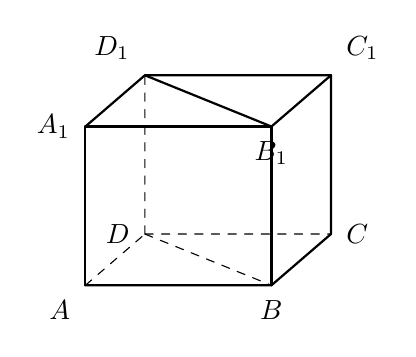
\begin{tikzpicture}[line cap=round, line join=round, scale=1.05]
\coordinate (A) at (0,0); \coordinate (B) at (2.25,0);
\coordinate (D) at (.72,.62); \coordinate (C) at (2.97,.62);
\coordinate (A1) at (0,1.92); \coordinate (B1) at (2.25,1.92);
\coordinate (D1) at (.72,2.54); \coordinate (C1) at (2.97,2.54);
% Solid visible cube edges
\draw[thick] (A)--(B)--(C);
\draw[thick] (A)--(A1)--(B1)--(B);
\draw[thick] (B1)--(C1)--(C);
\draw[thick] (A1)--(D1)--(C1);
\draw[thick] (C)--(C1);
% Hidden cube edges and hidden diagonal of BB1D1D
\draw[dashed] (A)--(D) (D)--(C) (D)--(D1);
\draw[dashed] (D)--(B);
% Visible diagonal of BB1D1D
\draw[thick] (D1)--(B1);
\node[below left=2pt] at (A) {$A$};
\node[below=2pt] at (B) {$B$};
\node[right=2pt] at (C) {$C$};
\node[left=2pt] at (D) {$D$};
\node[left=2pt] at (A1) {$A_1$};
\node[below=2pt] at (B1) {$B_1$};
\node[above left=2pt] at (D1) {$D_1$};
\node[above right=2pt] at (C1) {$C_1$};
\end{tikzpicture}
\end{center}
\nopagebreak[4]
\Needspace{4\baselineskip}
\textbf{解析}

对角面 $BB_1D_1D$ 将正方体分成两个全等的直三棱柱。每个三棱柱的三角形截面是直角边长为 $a$、斜边长为 $\sqrt2a$ 的等腰直角三角形，棱柱长度为 $a$。

要使两块拼成四棱柱，按棱柱的共同纵向截面看，两个全等三角形必须沿一条完整边拼成四边形。沿斜边拼时，两三角形合成边长为 $a$ 的正方形；棱柱长度也为 $a$，所得就是正方体，被题目“不是正方体”排除。

\Needspace{5\baselineskip}
沿直角边拼时，若两个三角形的直角顶点落在公共边同一端，外轮廓退化成一个三角形，不能作为四棱柱的四边形截面。要形成凸四边形，两个直角顶点须位于公共边相反端；此时截面为平行四边形，邻边长分别为 $a$ 和 $\sqrt2a$。其面积是两三角形面积之和：
\nopagebreak[4]
\[
S_{\text{底}}=2\cdot\frac{a^2}{2}=a^2,
\]
\Needspace{5\baselineskip}
周长为
\nopagebreak[4]
\[
p=2(a+\sqrt2a).
\]
\Needspace{5\baselineskip}
棱柱长为 $a$，全面积等于两个底面面积加侧面积：
\nopagebreak[4]
\[
S_{\text{全}}=2S_{\text{底}}+pa
=2a^2+2(a+\sqrt2a)a
=(4+2\sqrt2)a^2.
\]
因此，在刚性、整侧面拼接成棱柱的通常几何含义下，排除正方体拼法后表面积唯一。

\gkanswer{答案：$(4+2\sqrt2)a^2$}

\end{answer}
\begin{answer}
\gksolhead{13}{}

\textbf{题目}：

从 $0,1,2,3$ 这四个数中选三个不同的数作为函数 $f(x)=ax^2+bx+c$ 的系数，可组成不同的一次函数共有 $\underline{\qquad}$ 个，不同的二次函数共有 $\underline{\qquad}$ 个。（用数字作答）

\Needspace{4\baselineskip}
\textbf{解析}

从 $0,1,2,3$ 中取互不相同的 $a,b,c$ 组成 $f(x)=ax^2+bx+c$。一次函数要求 $a=0$，之后 $b$ 有 $3$ 种、$c$ 有 $2$ 种，共 $3\cdot2=6$ 个。二次函数要求 $a\ne0$，$a$ 有 $3$ 种，$b$ 有 $3$ 种，$c$ 有 $2$ 种，共 $3\cdot3\cdot2=18$ 个。

\gkanswer{答案：一次函数 $6$ 个；二次函数 $18$ 个}

\end{answer}
\begin{answer}
\gksolhead{14}{}

\textbf{题目}：

若关于 $x$ 的不等式 $x^2-ax-a>0$ 的解集为 $(-\infty,+\infty)$，则实数 $a$ 的取值范围是 $\underline{\qquad}$。

\Needspace{4\baselineskip}
\textbf{解析}

\Needspace{5\baselineskip}
二次式 $x^2-ax-a$ 要对所有实数 $x$ 严格大于零。首项系数为正，故其判别式须小于零：
\nopagebreak[4]
\[
\Delta=(-a)^2-4(1)(-a)=a^2+4a<0.
\]
解 $a(a+4)<0$ 得 $-4<a<0$。端点对应有实根，不能取到。

\gkanswer{答案：$-4<a<0$}

\end{answer}
\gkpart{三、解答题}

\begin{answer}
\gksolhead{15}{}

\textbf{题目}：

设函数 $f(x)=\lg(2x-3)$ 的定义域为集合 $M$，函数 $g(x)=\sqrt{(x-3)(x-1)}$ 的定义域为集合 $N$。求：

（1） 集合 $M,N$；

（2） 集合 $M\cap N,M\cup N$。

\Needspace{4\baselineskip}
\textbf{解析}

\gksubpart{(1) 求 $M,N$}

对 $f(x)=\lg(2x-3)$，真数须满足 $2x-3>0$，故 $M=(3/2,+\infty)$。对 $g(x)=\sqrt{(x-3)(x-1)}$，须 $(x-3)(x-1)\ge0$，故 $N=(-\infty,1]\cup[3,+\infty)$。

\gksubpart{(2) 求交集与并集}

按端点包含关系作交、并集即得结果。

\gkanswer{答案（1）：$M=(\frac32,+\infty)$，$N=(-\infty,1]\cup[3,+\infty)$}

\gkanswer{答案（2）：$M\cap N=[3,+\infty)$，$M\cup N=(-\infty,1]\cup(\frac32,+\infty)$}

\end{answer}
\begin{answer}
\gksolhead{16}{}

\textbf{题目}：

如图，正三棱锥 $S-ABC$ 中，底面边长是 $3$，棱锥的侧面积等于底面积的 $2$ 倍，$M$ 是 $BC$ 的中点。求：

（1） $\dfrac{AM}{SM}$ 的值；

（2） 二面角 $S-BC-A$ 的大小；

（3） 正三棱锥 $S-ABC$ 的体积。
\nopagebreak[4]
\begin{center}% Source-page vector redraw from 2005 Spring Beijing Arts, printed p. 215, Q16.
% Schematic placement only; no lengths or angles are encoded.
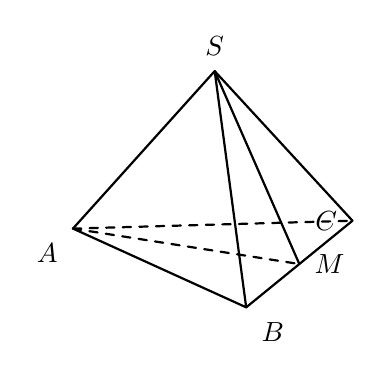
\begin{tikzpicture}[line cap=round, line join=round, scale=1.0]
\coordinate (A) at (0,1.0); \coordinate (B) at (2.2,0);
\coordinate (C) at (3.55,1.1); \coordinate (S) at (1.8,3.0);
\coordinate (M) at (2.875,.55); % midpoint of BC
\draw[thick] (A)--(B)--(S)--cycle;
\draw[thick] (S)--(C)--(B);
\draw[dashed, thick] (A)--(C) (A)--(M);
\draw[thick] (S)--(M);
\foreach \P/\pos in {A/below left,B/below right,C/left,S/above,M/right}
  \node[\pos=2pt] at (\P) {$\P$};
\end{tikzpicture}
\end{center}
\nopagebreak[4]
\Needspace{4\baselineskip}
\textbf{解析}

\gksubpart{(1) 求 $AM/SM$}

\Needspace{5\baselineskip}
底面为边长 $3$ 的等边三角形，面积
\nopagebreak[4]
\[
S_{ABC}=\frac{3^2\sqrt3}{4}=\frac{9\sqrt3}{4}.
\]
\Needspace{5\baselineskip}
设侧面斜高为 $SM$。三块全等侧面的总面积为 $3\cdot\frac12\cdot3\cdot SM=\frac92SM$，题给侧面积等于底面积的两倍，因此
\nopagebreak[4]
\[
\frac92SM=2\cdot\frac{9\sqrt3}{4},\qquad SM=\sqrt3.
\]
因 $M$ 是 $BC$ 中点，$AM$ 为等边三角形的中线，故 $AM=3\sqrt3/2$，于是 $AM/SM=3/2$。

\gksubpart{(2) 求二面角}

\Needspace{5\baselineskip}
令 $O$ 为底面中心，$SO\perp(ABC)$。中心到边 $BC$ 的距离为 $OM=\sqrt3/2$，在直角三角形 $SOM$ 中
\nopagebreak[4]
\[
SO=\sqrt{SM^2-OM^2}=\sqrt{3-\frac34}=\frac32.
\]
\Needspace{5\baselineskip}
二面角 $S-BC-A$ 的平面角为 $\angle SMO$，而 $A,M,O$ 共线，故其大小等于 $\angle SMA$。又 $AO=\sqrt3$，所以
\nopagebreak[4]
\[
AS=\sqrt{SO^2+AO^2}=\frac{\sqrt{21}}2.
\]
\Needspace{5\baselineskip}
在 $\triangle AMS$ 中由余弦定理，
\nopagebreak[4]
\[
\cos\angle AMS=\frac{AM^2+SM^2-AS^2}{2AM\cdot SM}=\frac12,
\]
故二面角为 $60^\circ$。

\gksubpart{(3) 求体积}

\Needspace{5\baselineskip}
最后
\nopagebreak[4]
\[
V=\frac13S_{ABC}\cdot SO
=\frac13\cdot\frac{9\sqrt3}{4}\cdot\frac32
=\frac{9\sqrt3}{8}.
\]

\gkanswer{答案（1）：$AM/SM=3/2$}

\gkanswer{答案（2）：$60^\circ$}

\gkanswer{答案（3）：$V=9\sqrt3/8$}

\end{answer}
\begin{answer}
\gksolhead{17}{}

\textbf{题目}：

\Needspace{5\baselineskip}
已知 $\{a_n\}$ 是等比数列，$a_1=2,a_4=54$；$\{b_n\}$ 是等差数列，且
\nopagebreak[4]
\[
b_1=2,\qquad b_1+b_2+b_3+b_4=a_1+a_2+a_3.
\]

（1） 求数列 $\{a_n\}$ 的通项公式及前 $n$ 项和 $S_n$ 的公式；

（2） 求数列 $\{b_n\}$ 的通项公式；

（3） 设 $U_n=b_1+b_4+b_7+\cdots+b_{3n-2}$，其中 $n=1,2,\ldots$，求 $U_{10}$ 的值。

\Needspace{4\baselineskip}
\textbf{解析}

\gksubpart{(1) 求 $a_n$ 与 $S_n$}

\Needspace{5\baselineskip}
由等比数列条件 $a_4=a_1q^3$ 得 $54=2q^3$，故 $q=3$，于是
\nopagebreak[4]
\[
a_n=2\cdot3^{n-1},\qquad S_n=\frac{2(3^n-1)}{3-1}=3^n-1.
\]

\gksubpart{(2) 求 $b_n$}

\Needspace{5\baselineskip}
又 $a_1+a_2+a_3=2+6+18=26$。设等差数列 $\{b_n\}$ 的公差为 $d$，则
\nopagebreak[4]
\[
b_1+b_2+b_3+b_4=8+6d=26,
\]
所以 $d=3$，$b_n=2+3(n-1)=3n-1$。

\gksubpart{(3) 求 $U_{10}$}

\Needspace{5\baselineskip}
在 $U_n=b_1+b_4+b_7+\cdots+b_{3n-2}$ 中，第 $j$ 项为
\nopagebreak[4]
\[
b_{3j-2}=3(3j-2)-1=9j-7.
\]
\Needspace{5\baselineskip}
这是首项 $2$、公差 $9$ 的等差数列，故
\nopagebreak[4]
\[
U_n=\frac n2\bigl(2+(9n-7)\bigr)=\frac{n(9n-5)}2,
\qquad U_{10}=425.
\]

\gkanswer{答案（1）：$a_n=2\cdot3^{n-1}$，$S_n=3^n-1$}

\gkanswer{答案（2）：$b_n=3n-1$}

\gkanswer{答案（3）：$U_{10}=425$}

\end{answer}
\begin{answer}
\gksolhead{18}{}

\textbf{题目}：

如图，$O$ 为坐标原点，过点 $P(2,0)$ 且斜率为 $k$ 的直线 $l$ 交抛物线 $y^2=2x$ 于 $M(x_1,y_1),N(x_2,y_2)$ 两点。

（1） 写出直线 $l$ 的截距式方程；

（2） 求 $x_1x_2$ 与 $y_1y_2$ 的值；

（3） 求证：$OM\perp ON$。
\nopagebreak[4]
\begin{center}% Source-page vector redraw from 2005 Spring Beijing Arts, printed p. 216, Q18.
% y^2=2x and the named secant/chord topology are source-visible; placement is schematic.
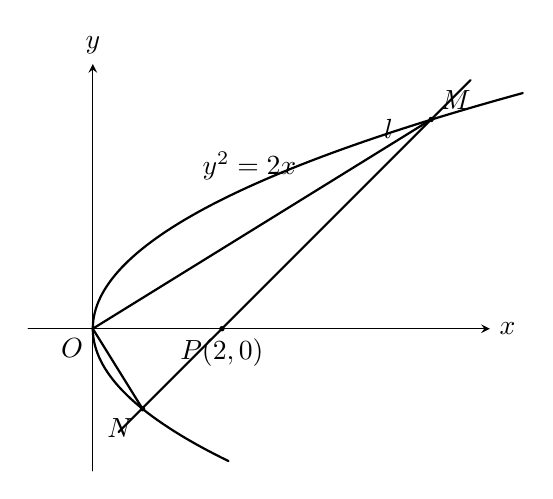
\begin{tikzpicture}[>=stealth, line cap=round, line join=round, scale=.82]
\draw[->] (-1.0,0)--(6.15,0) node[right] {$x$};
\draw[->] (0,-2.2)--(0,4.1) node[above] {$y$};
\node[below left] at (0,0) {$O$};
\draw[thick, domain=-2.05:3.65, samples=100, variable=\t]
  plot ({.5*\t*\t},{\t});
% A chord through the parabola's two marked points and the x-axis point P.
\coordinate (N) at (.77,-1.24); \coordinate (P) at (2,0); \coordinate (M) at (5.24,3.24);
\draw[thick] (.4,-1.6)--(5.85,3.85); % secant y=x-2 through P(2,0)
% Source also shows the two origin chords.
\draw[thick] (0,0)--(M) (0,0)--(N);
\fill (M) circle (1.2pt) (N) circle (1.2pt) (P) circle (1.2pt);
\node[above right] at (M) {$M$}; \node[below left] at (N) {$N$};
\node[below] at (P) {$P(2,0)$};
\node[above right] at (1.55,2.15) {$y^2=2x$};
\node[above left] at (4.8,2.8) {$l$};
\end{tikzpicture}
\end{center}
\nopagebreak[4]
\Needspace{8\baselineskip}

\Needspace{4\baselineskip}
\textbf{解析}

\gksubpart{(1) 写截距式}

\Needspace{5\baselineskip}
直线为 $l:y=k(x-2)$。题目给定它与抛物线交于两个不同点，因此 $k\ne0$；此时直线的截距式是
\nopagebreak[4]
\[
\frac{x}{2}-\frac{y}{2k}=1.
\]

\gksubpart{(2) 求 $x_1x_2$ 与 $y_1y_2$}

\Needspace{5\baselineskip}
把直线代入抛物线 $y^2=2x$：
\nopagebreak[4]
\[
k^2(x-2)^2=2x,
\]
\Needspace{5\baselineskip}
即
\nopagebreak[4]
\[
k^2x^2-(4k^2+2)x+4k^2=0.
\]
\Needspace{5\baselineskip}
设两交点为 $M(x_1,y_1)$、$N(x_2,y_2)$。韦达定理给出 $x_1x_2=4$；同时 $y_i=k(x_i-2)$，故
\nopagebreak[4]
\[
y_1y_2=k^2(x_1-2)(x_2-2)
=k^2\bigl(x_1x_2-2(x_1+x_2)+4\bigr)=-4.
\]

\gksubpart{(3) 证明垂直}

\Needspace{5\baselineskip}
于是
\nopagebreak[4]
\[
\overrightarrow{OM}\cdot\overrightarrow{ON}=x_1x_2+y_1y_2=4-4=0,
\]
所以 $OM\perp ON$。

边界说明：$k=0$ 时 $l$ 为 $y=0$，它与抛物线仅在顶点 $O$ 相交，并非两个不同交点。因此由题设“两点相交”隐含排除 $k=0$，推导中使用 $1/k$ 是有效的。

\gkanswer{答案（1）：$\frac{x}{2}-\frac{y}{2k}=1$（$k\ne0$）}

\gkanswer{答案（2）：$x_1x_2=4$，$y_1y_2=-4$}

\gkanswer{答案（3）：$OM\perp ON$}

\end{answer}
\begin{answer}
\gksolhead{19}{}

\textbf{题目}：

\Needspace{5\baselineskip}
经过长期观测得到：在交通繁忙的时段内，某公路段汽车的车流量 $y$（千辆/小时）与汽车的平均速度 $v$（千米/小时）之间的函数关系为
\nopagebreak[4]
\[
y=\frac{920v}{v^2+3v+1600}\quad(v>0).
\]

（1） 在该时段内，当汽车的平均速度 $v$ 为多少时，车流量最大？最大车流量为多少？（精确到 $0.1$ 千辆/小时）

（2） 若要求在该时段内车流量超过 $10$ 千辆/小时，则汽车的平均速度应在什么范围内？

\Needspace{4\baselineskip}
\textbf{解析}

\gksubpart{(1) 求最大车流量}

\Needspace{5\baselineskip}
记 $D(v)=v^2+3v+1600$。在 $v>0$ 上 $D(v)>0$。对
\nopagebreak[4]
\[
y=\frac{920v}{D(v)}
\]
\Needspace{5\baselineskip}
求导得
\nopagebreak[4]
\[
y'=\frac{920(1600-v^2)}{D(v)^2}.
\]
\Needspace{5\baselineskip}
所以 $0<v<40$ 时递增，$v>40$ 时递减，最大值在 $v=40$ 取得：
\nopagebreak[4]
\[
y_{\max}=\frac{920\cdot40}{40^2+3\cdot40+1600}
=\frac{36800}{3320}\approx11.0843,
\]
按题意精确到 $0.1$ 为 $11.1$ 千辆/小时。

\gksubpart{(2) 求流量超过 $10$ 的速度范围}

\Needspace{5\baselineskip}
因分母为正，$y>10$ 等价于
\nopagebreak[4]
\[
920v>10(v^2+3v+1600),
\]
\Needspace{5\baselineskip}
即 $v^2-89v+1600<0$。该二次式两根为
\nopagebreak[4]
\[
\frac{89\pm\sqrt{89^2-4\cdot1600}}2
=\frac{89\pm39}2=25,64,
\]
故 $25<v<64$ 千米/小时。

\gkanswer{答案（1）：在 $v=40$ 千米/小时取得，最大车流量约为 $11.1$ 千辆/小时}

\gkanswer{答案（2）：$25<v<64$ 千米/小时}

\end{answer}
\begin{answer}
\gksolhead{20}{}

\textbf{题目}：

\Needspace{5\baselineskip}
现有一组互不相同且从小到大排列的数据 $a_0,a_1,a_2,a_3,a_4,a_5$，其中 $a_0=0$。为提取反映数据间差异程度的某种指标，今对其进行如下加工：记
\nopagebreak[4]
\[
T=a_0+a_1+\cdots+a_5,\qquad x_n=\frac{n}{5},\qquad y_n=\frac{1}{T}(a_0+a_1+\cdots+a_n),
\]
作函数 $y=f(x)$，使其图象为逐点依次连接点 $P_n(x_n,y_n)$（$n=0,1,2,\ldots,5$）的折线。

（1） 求 $f(0)$ 和 $f(1)$ 的值；

（2） 设 $P_{n-1}P_n$ 的斜率为 $k_n$（$n=1,2,3,4,5$），判断 $k_1,k_2,k_3,k_4,k_5$ 的大小关系；

（3） 证明：$f(x_n)<x_n$（$n=1,2,3,4$）。

\Needspace{4\baselineskip}
\textbf{解析}

\gksubpart{(1) 求端点函数值}

令 $T=a_0+a_1+\cdots+a_5$。题设 $a_0=0$ 且各增量为正，故 $T>0$。折线首末端点为 $P_0=(0,0)$ 与 $P_5=(1,1)$，因此 $f(0)=0,f(1)=1$。

\gksubpart{(2) 比较斜率}

\Needspace{5\baselineskip}
每段横坐标增量为 $1/5$，纵坐标增量为 $a_n/T$，故
\nopagebreak[4]
\[
k_n=\frac{a_n/T}{1/5}=\frac{5a_n}{T}.
\]
由 $a_1<a_2<a_3<a_4<a_5$ 且 $T>0$，得到 $k_1<k_2<k_3<k_4<k_5$。

\gksubpart{(3) 证明节点不等式}

\Needspace{5\baselineskip}
在 $x_n=n/5$ 处，
\nopagebreak[4]
\[
f(x_n)=\frac{a_1+\cdots+a_n}{T},
\]
\Needspace{5\baselineskip}
故只需证明 $nT-5(a_1+\cdots+a_n)>0$。令 $S_n=a_1+\cdots+a_n$，$R_n=a_{n+1}+\cdots+a_5$。对 $1\le n\le4$，有 $S_n\le na_n$ 且 $R_n>(5-n)a_n$，所以
\nopagebreak[4]
\[
nT-5S_n=nR_n-(5-n)S_n>n(5-n)a_n-(5-n)na_n=0.
\]
因此 $f(x_n)<x_n$（$n=1,2,3,4$）。

\gkanswer{答案（1）：$f(0)=0$，$f(1)=1$}

\gkanswer{答案（2）：$k_1<k_2<k_3<k_4<k_5$}

\gkanswer{答案（3）：$f(x_n)<x_n$（$n=1,2,3,4$）}

\end{answer}